\documentclass[a4paper, 12pt]{article}%тип документа



%отступы
\usepackage[left=1cm,right=1cm,top=1cm,bottom=2cm,bindingoffset=0cm]{geometry}

%%% Работа с русским языком
\usepackage{graphicx}
\usepackage{cmap}                           % поиск в PDF
\usepackage{mathtext} 			 	       % русские буквы в формулах
\usepackage[T2A]{fontenc}               % кодировка
\usepackage[utf8]{inputenc}              % кодировка исходного текста
\usepackage[english,russian]{babel} 
\usepackage{float}

\usepackage[export]{adjustbox} % локализация и переносы

\usepackage{subfig}% http://ctan.org/pkg/subfig
\usepackage{booktabs}

\usepackage{wrapfig}


%Матеша
\usepackage{amsmath,amsfonts,amssymb,amsthm,mathtools} % AMS
\usepackage{icomma} % "Умная" запятая

%\mathtoolsset{showonlyrefs=true} % Показывать номера только у тех формул, на которые есть \eqref{} в тексте.

%% Шрифты
\usepackage{euscript}	 % Шрифт Евклид
\usepackage{mathrsfs} % Красивый матшрифт

%% Свои команды
\DeclareMathOperator{\sgn}{\mathop{sgn}}

%% Перенос знаков в формулах (по Львовскому)
\newcommand*{\hm}[1]{#1\nobreak\discretionary{}
	{\hbox{$\mathsurround=0pt #1$}}{}}




\author{Гаврилин Илья Дмитриевич \\
	Б01-101}
\title{\textbf{Работа 2.3.1 \\ 
		Поучение и измерение вакуума}}

\begin{document}
		\maketitle
	\section{Аннотация}
	В ходе этой работы происходит обучение работы с форвакуумным и диффузионным насосом, для получения вакуума различной глубины. Находится максимальная глубина вакуума, достижимая на конкретной установке, измеряются объемы форвакуумного и высоковакуумного баллона.
	Изучается процесс создания искусственной течи между частями установки, определяется скорость откачки системы в стационарном режиме, а также ухудшение и улучшение вакуума.
	\section{Теоретические сведения}
	\subsection{Схема работы экспериментальной установки}
	В данной работе используются традиционные методы откачки механическим форвакуумным насосом до давления $10^{-2}$ торр и диффузионным масляным до давления $10^{-4}$ торр. Установка изготовлена из стекла, и состоит из форвакуумного баллона (ФБ), высоковакуумного диффузионного насоса (ВН), 
	высоковакуумного баллона (ВБ), масляного (М) и ионизационного (И) манометров, термопарных манометров ($M_{1}$ и $M_{2}$), форвакуумного насоса (ФН) и соединительных кранов ($K_{1}$, $K_{2}$, ..., $K_{6}$) (рис. 1).\linebreak
	\begin{figure}[h]
		\centering
		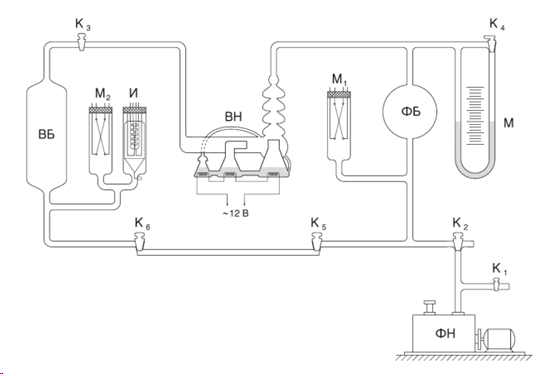
\includegraphics[width=0.6\linewidth]{screenshot001}
		\caption{Схема экспериментальной установки}
	\end{figure}

	Следует учитывать что некоторые части установки, такие как диффузионный насос и ионизационный манометр имеют ограничения по рабочему давлению, следует проверять по термопарным манометрам допустимые границы включения оборудования, написанные в характеристиках каждой установки. (В среднем $10^{-2} - 10^{-4}$ мм.рт.ст.)
	\subsection{Откачка воздуха}
	Опишем процесс откачки математически: \\
	Пусть W --- объем газа, удаляемого из сосуда при данном давлении за единицу времени, $Q_i$ для различных значений $i$ обозначим различные притоки газа в сосуд (в единицах $PV$), такие как течи извне $Q_\text{и}$, десорбция с поверхностей внутри сосуда $Q_\text{д}$, обратный ток через насос $Q_\text{н}$. Тогда, приравнивая убыль газа из сосуда (с точностью до $RT/\mu$) в единицу времени $-VdP$ и сумму перечисленных токов имеем:
\begin{equation}
	-VdP = (PW - \sum_i Q_i)dt
\end{equation}
При достижении предельного вакуума устанавливается давление $P_{\text{пр}}$, и $dP = 0$. Тогда
\begin{equation}
	W = ( \sum_i Q_i )/P_{\text{пр}}
\end{equation}
Поскольку обычно $Q_\text{и}$ постоянно, а $Q_\text{н}$ и $Q_\text{д}$ слабо зависят от времени, также считая постоянной W, можем проинтегрировать (1) и получить:
\begin{equation}
	P - P_{\text{пр}} = (P_0 - P_{\text{пр}})\exp(-\frac{W}{V}t)
\end{equation}
Полная скорость откачки $W$, собственная скорость откачки насоса $W_{\text{н}}$ и проводимости элементов системы $C_1, C_2,...$ соотносятся согласно формуле (4), и это учтено в конструкции установки.
\begin{equation}
	\frac{1}{W} = \frac{1}{W} + \frac{1}{C_1} + \frac{1}{C_2} + ...
\end{equation}
\subsection{Течение газа по трубкам}
Характер течения газа существенно зависит от соотношения между размерами системы и длиной свободного пробега молекул. При атмосферном и форвакуумном давлениях  длина свободного пробега меньше диаметра трубок, и течение газа определяется его вязкостью, т.е. взаимодействием молекул. При высоком вакууме течение существеннее определяется взаимодействием со стенками \\
Для количества газа, протекающего через трубу длины $l$ и радиуса $r$ в условиях высокого вакуума, справедлива формула:
\begin{equation}
	\frac{d(PV)}{dt} = \frac{4}{3}r^3\sqrt{\frac{2\pi RT}{\mu}}\frac{P_2 - P_1}{l}
\end{equation}
Если труба соединяет насос установку, то давлением $P_1$ у насоса можно пренебречь. Давление в сосуде $P = P_2$. Тогда имеем:
\begin{equation}
	C_\text{тр} = \left(\frac{dV}{dt}\right)_\text{тр} = \frac{4r^3}{3l}\sqrt{\frac{2\pi RT}{\mu}}
\end{equation}
\section{Ход работы}
\subsection{Измерение параметров установки}
Проверим правильность расположения кранов на установке, запишем важные параметры, связанные с установкой.\\
\begin{equation*}
	\rho_{масла} = 0.885 ~г/см^{3}, V_{зап} = 50 ~см^{3}  d_{кап} = 0.8~мм.
\end{equation*}
Также, стоит замерить атмосферное давление: $P_{атм}=99.7~кПа$
\subsection{Замер объемов баллонов}
Откачаем из установки воздух, предварительной создав "запертый" объем. Запишем значение давления, полученное по термопарному манометру: $P_{ост} = (2.1 \pm 0.1)*10^{-2}~мм. ~рт.~ст.$\\
\begin{equation*}
		h_1 = (13.4 \pm 0.1)~см~масл. ~ст.,\quad  h_2 = (39.3 \pm 0.1)~ см ~масл. ~ст.,
\end{equation*}

\begin{equation*}
	\sigma_{\Delta h} = \sqrt{\sigma_{\Delta h1}^2 + \sigma_{\Delta h2}^2}\approx 0.2~ см. ~масл. ~ст. \quad \Delta h_{фв} = (25.9 \pm 0.2) ~ см ~масл. ~ст.
\end{equation*}
Зная объём "запертой"  части установки $V_{кап} = 50 ~ см^3$  и используя соотношение $P_1/P_2=V_2/V_1$ (считаем температуру постоянной) вычислим объём форвакуумной части установки. При этом давление $P_1 = P_{атм} = (99.7 \pm 0.05) ~ кПа$ $P_2 = \Delta h_{фв}  \rho_{масл} g + P_{ост}$, а относительная погрешность полученного значения равна относительной погрешности величины $\Delta h_{фв} $:
\begin{equation*}
	V_{фв} = (2214\pm 17) ~см^{3}
\end{equation*}
Проведем аналогичные замеры только для случая, когда к системе добавляется высоковакуумный баллон.
\begin{equation*}
	h_3 = (18.4 \pm 0.1)~см~масл. ~ст.,\quad  h_4 = (35.2 \pm 0.1)~ см ~масл. ~ст.,
\end{equation*}
\begin{equation*}
	\sigma_{\Delta h} = \sqrt{\sigma_{\Delta h1}^2 + \sigma_{\Delta h2}^2}\approx 0.15~ см. ~масл. ~ст. \quad \Delta h_{фв} = (16.80 \pm 0.15) ~ см ~масл. ~ст.
\end{equation*}
При расчете давления по формуле использованной в первом случае, учтем, что: $V_{вв} = V_{2} - V_{фв}$
\begin{equation*}
	V_{вв} = (1199\pm 10) ~см^{3}
\end{equation*}

\subsection{Получение высокого вакуума, измерение скорости откачки}
При достаточно низком давлении запустим диффузионный насос, ионизационный манометр(проведя процедуры по накалу и дегазации). Подождав 10-15 минут, замерим предельное возможное для конкретной установки давление: $P_{пр}=4.1\cdot10^{-5}~мм.~рт.~ст.$\\
Создадим искуственную течь, соединив капиляром форвакуумную и высоковакуумную часть установки, при этом у нас получится установившееся давление, когда скорость откачки насоса уравновесит поток из искусственной течи: $P_{уст}=1.1\cdot10^{-4}~мм.~рт.~ст.$\\
Открыв капилляр замерим ухудшение вакуума, после закрытия капиляра измерим улучшение вакуума, представим данные в виде таблицы и графика(табл. 1, 2).\\
\begin{table}[H]
	\centering
	\begin{tabular}{|c|c|c|c|}
		\hline
		t, сек & P, $\cdot 10^{-5}$ мм. рт. ст. & t, сек & P, $\cdot 10^{-5}$ мм. рт. ст. \\ \hline
		0      & 3.9                                & 55     & 31.0                               \\ \hline
		5      & 4.8                                & 60     & 34.0                               \\ \hline
		10     & 5.0                                & 65     & 37.0                               \\ \hline
		15     & 5.5                                & 70     & 40.0                               \\ \hline
		20     & 8.6                                & 75     & 43.0                               \\ \hline
		25     & 12.0                               & 80     & 46.0                               \\ \hline
		30     & 16.0                               & 85     & 49.0                               \\ \hline
		35     & 19.0                               & 90     & 52.0                               \\ \hline
		40     & 22.0                               & 95     & 55.0                               \\ \hline
		45     & 25.0                               & 100    & 57.0                               \\ \hline
		50     & 28.0                               & 105    & 60.0                               \\ \hline
	\end{tabular}
	\caption{ухудшение вакуума при образовании течи}
\end{table}
\begin{figure}[H]
	\centering
	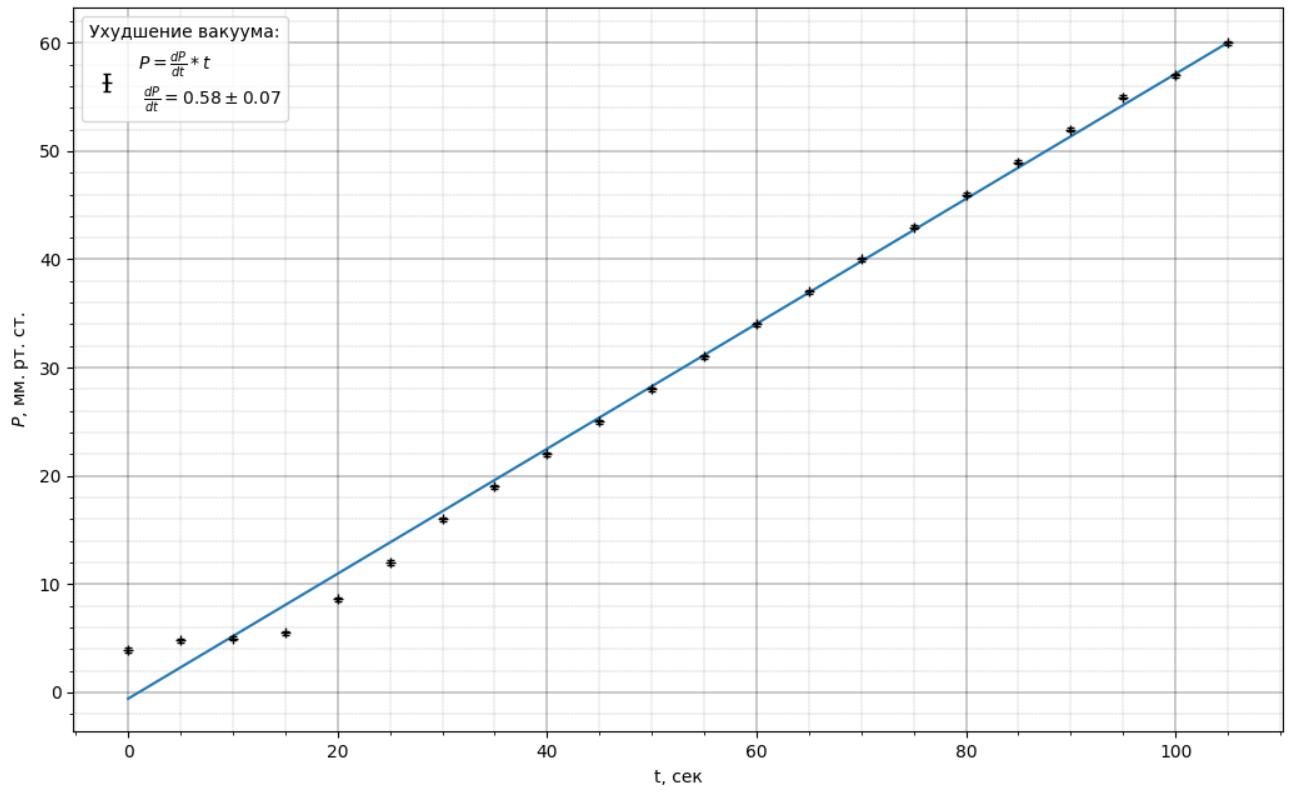
\includegraphics[width=1\linewidth]{graph2}
	\caption[]{зависимость давления от времени при ухудшении вакуума}
	\label{fig:graph2}
\end{figure}
    \begin{figure}[H]
	\centering
	\subfloat[Таблица 2: улучшение вакуума при устранении течи]{
		\adjustbox{valign=b}{\begin{tabular}{|c|c|c|}
			\hline
			t, сек & P, $\cdot 10^{-5}$ мм. рт. ст. & $ln(P/P_{0})$       \\ \hline

			0                        & 56                       & 0.00                          \\ \hline
			1                        & 41                       & -0.31                         \\ \hline
			2                        & 30                       & -0.62                         \\ \hline
			3                        & 22                       & -0.93                         \\ \hline
			4                        & 17                       & -1.19                         \\ \hline
			5                        & 13.2                     & -1.45                         \\ \hline
			6                        & 10.4                     & -1.68                         \\ \hline
			7                        & 8.4                      & -1.90                         \\ \hline
			8                        & 6.9                      & -2.09                         \\ \hline
			9                        & 5.5                      & -2.32                         \\ \hline
			10                       & 4.2                      & -2.59                         \\ \hline
		\end{tabular}}
		
		\label{res-ma}}
	\subfloat[Рис: зависимость логарифма частного давлений от времени]{           
			
	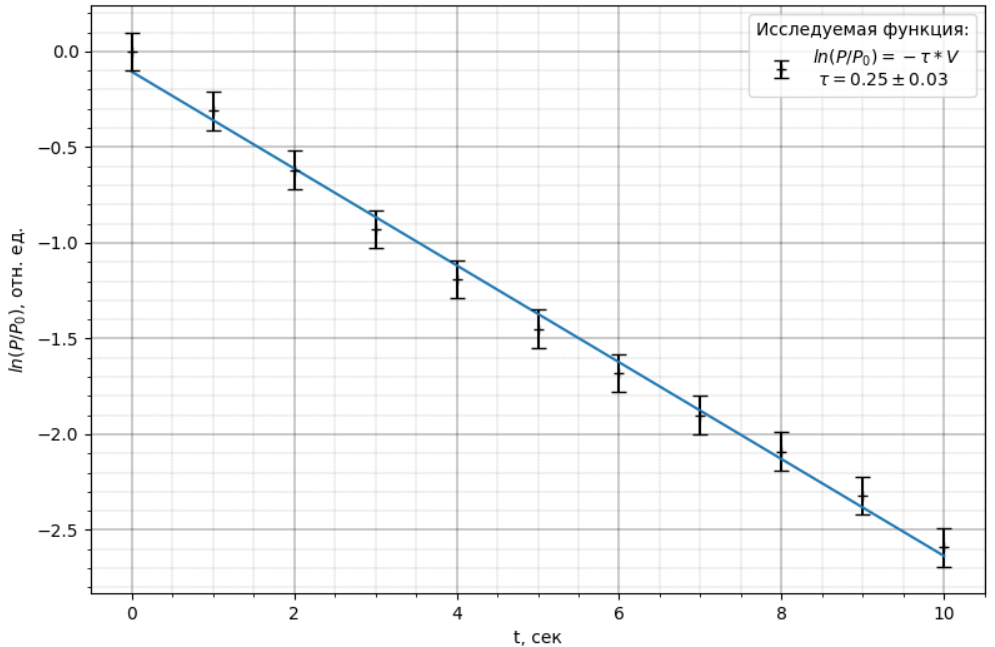
\includegraphics[width=0.6\linewidth]{Снимок экрана 2022-03-20 211422}
	} 
		\label{fig:ma}          
	\caption{Улучшение вакуума}
	\end{figure}
\textit{На рис. 2 можем заметить, что первые 6-7 точек плохо ложатся на интерполяционную кривую, вероятнее всего это связано с процессом изменения конфигурации кранов и не ламинарным течением газа в капиллярах.}
\subsection{Рассчет производительности насоса и пропускной способности капиляра}
Сначала проведём вычисления для коэффициента $\tau$, полученного при улучшении вакуума (для этого мы строили графики зависимости $\ln (P/P_0)$ от $t$). Поскольку $W = -\tau V_{вв}$, то $\varepsilon_W = \sqrt{\varepsilon_k^2 + \varepsilon_{V_{вв}}^2} \approx 4\%$, в результате имеем: 

\begin{equation*}
W = (0.299 \pm 0.011) ~ л /	 с.
\end{equation*}
Оценим величину потока газа  $Q_Н$. Для этого воспользуемся данными, полученными при ухудшении вакуума. А именно построим графики зависимости $P(t)$ и определим для них коэффициенты угла наклона прямой. Поскольку $V_{вв}dP = (Q_Д + Q_И) dt$ получим $)(Q_Д + Q_И) = \frac{dP}{dt}V_{вв} = (0.69 \pm 0.04)~ \cdot 10^{-5} ~торр \cdot л / c $ (Погрешность рассчитывается по формуле $\varepsilon =  \sqrt{\varepsilon_k^2 + \varepsilon_{V_{вв}}^2} \approx 6\%$). Используя формулу $Q_Н = P_{пр}W - (Q_Д + Q_И)$, а значит $\varepsilon_{Q_Н} =  \sqrt{\varepsilon_{P_{пр}W}^2 + \varepsilon^2} \approx 9\%$ получим, что: 

\begin{equation*}
	Q_Н = (0.54 \pm 0.05) \cdot 10^{-5} ~ торр \cdot л / с.
\end{equation*}
\textbf{Оценим пропускную способность трубки по ф-ле (6):}
\begin{equation*}
	L = (10.8 \pm 0.1)~ см; \quad   d = (0.8 \pm 0.1) ~ мм.
\end{equation*}

\begin{equation*}
	C_{тр} = (5.8 \pm 0.3)\cdot 10^{-3}~ л / с.
\end{equation*}


Погрешность $C_{тр}$  оценена как корень из суммы квадратов погрешностей длинны и диаметра (которые явным образом не указаны на установке, поэтому считаем что замер длины проведен линейкой, а замер диаметра штангенциркулем, погрешность может оказаться завышенной). \\
\textbf{При установлении течи мы замерили установившееся давление в двух баллонах:}
\begin{equation*}
	P_{уст} = (1.1 \pm 0.1) \cdot 10^{-4} ~ торр.;	P_{фв} = (3.4 \pm 0.1) \cdot 10^{-3} ~ торр.
\end{equation*}

\textbf{С помощью полученных данных можем посчитать W другим способом:}
$$
P_{пр} W = Q_1, \quad P_{уст} W = Q_1 + \frac{d(PV)_{кап}}{dt}, 
$$

то 

$$
W = C_{тр}\cdot \frac{P_{фв}}{P_{ уст}-P_{пр}} = 0.28 \pm 0.05 ~л / c;
$$


(Поскольку давления измерены с точностью не менее $10\%$, то можно учитывать погрешность, вносимую величиной $\frac{d(PV)_{кап}}{dt}$ относительная погрешность которой равна относительной погрешности $C_{тр}$, то есть составляет $20\%$)
\section{Вывод}
В ходе работы была изучена работа установки по получению среднего и высокого вакуума. Приобретены навыки работы с вакуумными установками. Проведена работа по имитации течи из высоковакуумного баллона, за счет этого измерена производительность насоса двумя методами:\\
1) Уравновешивание поступающего и откачиваемого из баллона воздуха. $W = 0.28 \pm 0.05 ~л / c $\\
2) Рассчет по ухудшению и улучшению вакуума. $W = 0.299 \pm 0.011 ~л / c $\\
В ходе опыта доказана справедливость обоих методов подсчета.

\end{document}
